\documentclass{article}
\PassOptionsToPackage{numbers,compress}{natbib}
\usepackage[preprint]{neurips_2025}
\usepackage[utf8]{inputenc}
\usepackage[T1]{fontenc}
\usepackage{hyperref}
\usepackage{url}
\usepackage{booktabs}
\usepackage{amsmath}
\usepackage{graphicx}
\usepackage{microtype}
\usepackage{xcolor}

\title{Generating Paintings with a Deep Convolutional GAN on WikiArt}

\author{S.~Ananth \\ ECE 285, Homework 2 \\ University of California, San Diego}

\begin{document}
\maketitle

\begin{abstract}
We train a deep convolutional generative adversarial network (DCGAN) to synthesize $64\times64$ paintings from the WikiArt dataset. Trained for 100 epochs on 81.4k paintings, the best generator reaches FID $15.5$ (standard pool3 features; $0.0192$ with the PyTorch-Ignite default) and Inception Score $2.99$ on 50k samples, a $4.3\times$ FID improvement over a baseline trained on an 18k-image subset.
\end{abstract}

\section{Method}
\paragraph{Data.} WikiArt~\cite{wikiart} contains $\sim$81k paintings across 27 styles. As the Kaggle archive (31\,GB) exceeded our storage quota, we streamed the same collection shard by shard from its Hugging Face mirror (\texttt{huggan/wikiart}): all 72 shards (81.4k images) for the main run, 16 shards (18{,}099) for a baseline. Images were center-cropped, resized to $64\times64$, scaled to $[-1,1]$ and randomly flipped.

\paragraph{Model.} We follow DCGAN~\cite{dcgan}. The generator maps $z\sim\mathcal{N}(0,I_{100})$ through five transposed convolutions ($4\times4$ kernels, stride 2; channels $512\!\to\!256\!\to\!128\!\to\!64\!\to\!3$) with BatchNorm+ReLU and a final $\tanh$ (3.58M parameters). The discriminator mirrors it with strided convolutions, BatchNorm and LeakyReLU(0.2), ending in a single logit (2.77M parameters). Weights are initialized from $\mathcal{N}(0,0.02)$. We use the non-saturating GAN loss~\cite{gan}: $\mathcal{L}_D=-\log D(x)-\log(1-D(G(z)))$, $\mathcal{L}_G=-\log D(G(z))$, with one-sided label smoothing (real target 0.9).

\begin{table}[h]
\centering
\caption{Hyperparameters of the main run (the baseline differs only in data and length).}
\label{tab:hp}
\small
\begin{tabular}{ll@{\hspace{2.5em}}ll}
\toprule
Image size & $64\times64\times3$ & Optimizer (G and D) & Adam, $\beta_1{=}0.5$, $\beta_2{=}0.999$ \\
Training images & 81.4k & Learning rate (G and D) & $2\times10^{-4}$ \\
Latent dimension & 100 & Batch size & 128 \\
Base width ($n_{gf}$, $n_{df}$) & 64, 64 & Epochs / iterations & 100 / 63{,}600 \\
Real-label smoothing & 0.9 & D:G updates; time & 1:1; 79\,min on one GPU \\
\bottomrule
\end{tabular}
\end{table}

\section{Results}
\paragraph{Training dynamics.} Training never diverges (Figure~\ref{fig:curves}). Short spikes near epochs 45 and 80 recover quickly. Until epoch $\sim$30 the players are balanced ($D(x)\approx0.73$, $D(G(z))\approx0.17$). Afterwards the discriminator slowly gains the upper hand ($D(x)\to0.84$, $D(G(z))\to0.07$, $\mathcal{L}_G$: $3\to4$), which coincides with the FID plateau.

\begin{figure}[h]
\centering
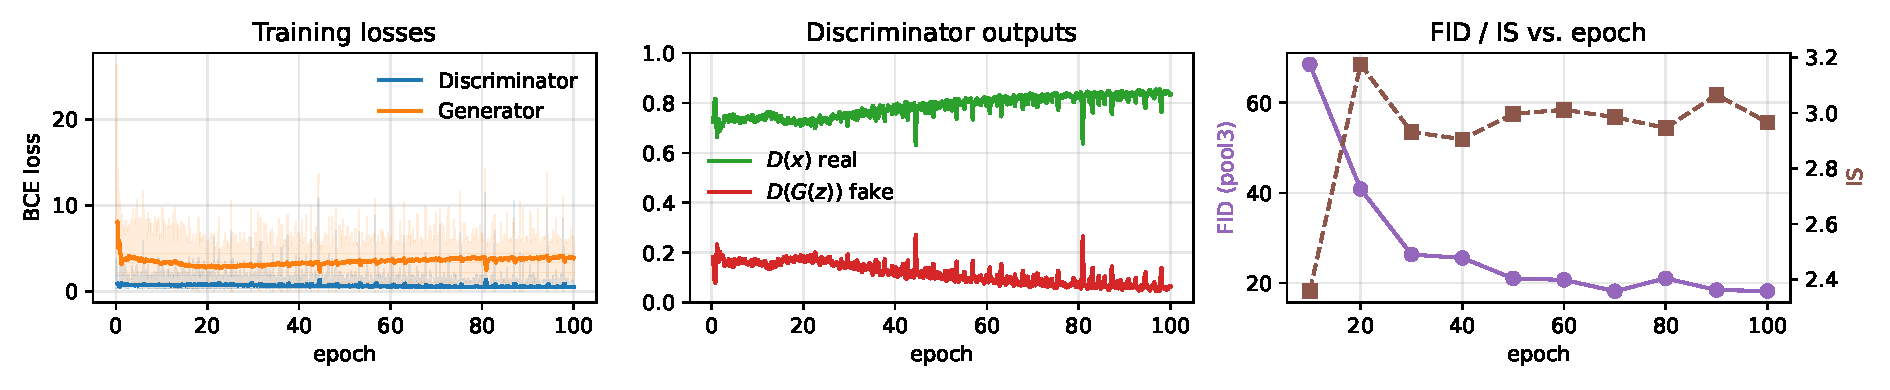
\includegraphics[width=\linewidth]{figs_full/curves.pdf}
\caption{Main run. Left: losses (light: per iteration; dark: 212-iteration average). Middle: mean $D$ output on real and fake batches. Right: pool3 FID ($\downarrow$) and IS ($\uparrow$) per checkpoint (10k samples).}
\label{fig:curves}
\end{figure}

\paragraph{Quantitative evaluation.} We compute FID~\cite{fid} and IS~\cite{is} with the PyTorch-Ignite code~\cite{ignite}, upsampling images bilinearly to $299\times299$. Ignite's default \texttt{FID} uses Inception's 1000-d \emph{softmax probabilities}, so its values are far smaller than published FIDs. We therefore also report the standard FID on 2048-d pool3 features. Each checkpoint was scored on 10k samples, and the best one (epoch 70) was re-scored on 50k (Table~\ref{tab:metrics}). FID plateaus from epoch 70, where differences fall within sampling noise. IS settles near 3.0. Real paintings score only 3.92 because they fit ImageNet classes poorly, so FID is the more informative metric.

\begin{table}[h]
\centering
\caption{Main run per checkpoint (10k samples) and best checkpoint (50k). Baseline: 50 epochs, 5k samples.}
\label{tab:metrics}
\small
\setlength{\tabcolsep}{4pt}
\begin{tabular}{lccccccc|ccc}
\toprule
Epoch & 10 & 20 & 30 & 50 & 70 & 90 & 100 & 70 (50k) & Baseline & Real \\
\midrule
FID, pool3 $\downarrow$ & 68.5 & 40.8 & 26.3 & 21.0 & 18.2 & 18.4 & 18.2 & \textbf{15.5} & 67.3 & -- \\
FID, Ignite $\downarrow$ & .0700 & .0409 & .0286 & .0250 & .0223 & .0205 & .0215 & \textbf{.0192} & .0699 & -- \\
IS $\uparrow$ & 2.36 & 3.17 & 2.93 & 3.00 & 2.98 & 3.07 & 2.97 & \textbf{2.99} & 2.44 & 3.92 \\
\bottomrule
\end{tabular}
\end{table}

\paragraph{Effect of data.} After 10 epochs the main run has taken about as many steps as the whole baseline (6.4k vs.\ 7.1k) and scores about the same (FID 68.5 vs.\ 67.3). The $4.3\times$ gain therefore comes from continued training on a larger, more diverse dataset.

\begin{figure}[h]
\centering
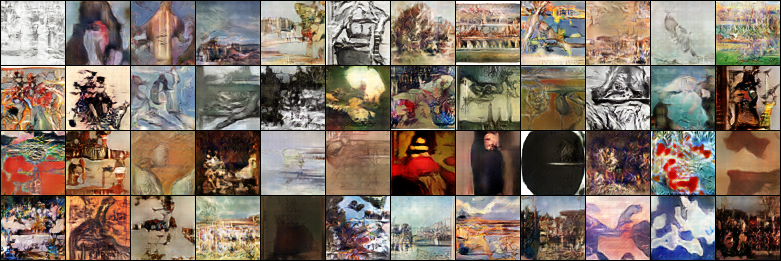
\includegraphics[height=1.08in]{figs_full/fake.png}\hfill
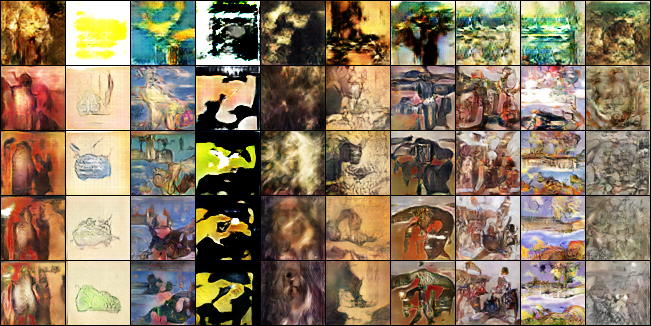
\includegraphics[height=1.08in]{figs_full/progress.png}
\caption{Left: 48 random samples from the best (epoch-70) generator. Right: 10 fixed latent vectors decoded at epochs 10, 30, 50, 80, 100 (rows, top to bottom).}
\label{fig:samples}
\end{figure}

\paragraph{Generated images.} Samples (Figure~\ref{fig:samples}) span WikiArt's styles: ink sketches, impressionist landscapes, dark seated figures, portrait-like faces and colorful expressionist scenes with brush-stroke texture. They are much sharper than the baseline's blurry color fields, with no mode collapse. Across epochs each latent vector keeps its palette and layout while gaining detail. Objects remain only suggestive, and faint checkerboard artifacts persist.

\paragraph{Discussion.} Data was the strongest lever. As FID plateaus after epoch 70, further gains likely need method changes (generator EMA, spectral normalization, TTUR, upsample+conv layers, genre conditioning). Inception metrics, built for photographs, are an imperfect judge of art.

{\footnotesize
\setlength{\itemsep}{0pt}\setlength{\parskip}{0pt}
\begin{thebibliography}{9}\setlength{\itemsep}{0pt}
\bibitem{wikiart} WikiArt dataset. \url{https://www.kaggle.com/datasets/steubk/wikiart}.
\bibitem{dcgan} A.~Radford et al. Unsupervised representation learning with deep convolutional GANs. \emph{ICLR}, 2016.
\bibitem{gan} I.~Goodfellow et al. Generative adversarial nets. \emph{NeurIPS}, 2014.
\bibitem{fid} M.~Heusel et al. GANs trained by a two time-scale update rule converge to a local Nash equilibrium. \emph{NeurIPS}, 2017.
\bibitem{is} T.~Salimans et al. Improved techniques for training GANs. \emph{NeurIPS}, 2016.
\bibitem{ignite} PyTorch-Ignite. GAN evaluation with FID and IS. \url{https://pytorch-ignite.ai/blog/gan-evaluation-with-fid-and-is/}.
\end{thebibliography}
}

\end{document}
